% This is "sig-alternate.tex" V2.1 April 2013
% This file should be compiled with V2.5 of "sig-alternate.cls" May 2012
%
% This example file demonstrates the use of the 'sig-alternate.cls'
% V2.5 LaTeX2e document class file. It is for those submitting
% articles to ACM Conference Proceedings WHO DO NOT WISH TO
% STRICTLY ADHERE TO THE SIGS (PUBS-BOARD-ENDORSED) STYLE.
% The 'sig-alternate.cls' file will produce a similar-looking,
% albeit, 'tighter' paper resulting in, invariably, fewer pages.
%
% ----------------------------------------------------------------------------------------------------------------
% This .tex file (and associated .cls V2.5) produces:
%       1) The Permission Statement
%       2) The Conference (location) Info information
%       3) The Copyright Line with ACM data
%       4) NO page numbers
%
% as against the acm_proc_article-sp.cls file which
% DOES NOT produce 1) thru' 3) above.
%
% Using 'sig-alternate.cls' you have control, however, from within
% the source .tex file, over both the CopyrightYear
% (defaulted to 200X) and the ACM Copyright Data
% (defaulted to X-XXXXX-XX-X/XX/XX).
% e.g.
% \CopyrightYear{2007} will cause 2007 to appear in the copyright line.
% \crdata{0-12345-67-8/90/12} will cause 0-12345-67-8/90/12 to appear in the copyright line.
%
% ---------------------------------------------------------------------------------------------------------------
% This .tex source is an example which *does* use
% the .bib file (from which the .bbl file % is produced).
% REMEMBER HOWEVER: After having produced the .bbl file,
% and prior to final submission, you *NEED* to 'insert'
% your .bbl file into your source .tex file so as to provide
% ONE 'self-contained' source file.
%
% ================= IF YOU HAVE QUESTIONS =======================
% Questions regarding the SIGS styles, SIGS policies and
% procedures, Conferences etc. should be sent to
% Adrienne Griscti (griscti@acm.org)
%
% Technical questions _only_ to
% Gerald Murray (murray@hq.acm.org)
% ===============================================================
%
% For tracking purposes - this is V2.0 - May 2012
\documentclass{sig-alternate-05-2015}
\usepackage{hyperref}

% remove copyright space
\makeatletter
\def\@copyrightspace{\relax}
\makeatother

\begin{document}

% --- Author Metadata here ---
%\CopyrightYear{2007} % Allows default copyright year (20XX) to be over-ridden - IF NEED BE.
%\crdata{0-12345-67-8/90/01}  % Allows default copyright data (0-89791-88-6/97/05) to be over-ridden - IF NEED BE.
% --- End of Author Metadata ---

\title{CS388: Assignment-2}
%
% You need the command \numberofauthors to handle the 'placement
% and alignment' of the authors beneath the title.
%
% For aesthetic reasons, we recommend 'three authors at a time'
% i.e. three 'name/affiliation blocks' be placed beneath the title.
%
% NOTE: You are NOT restricted in how many 'rows' of
% "name/affiliations" may appear. We just ask that you restrict
% the number of 'columns' to three.
%
% Because of the available 'opening page real-estate'
% we ask you to refrain from putting more than six authors
% (two rows with three columns) beneath the article title.
% More than six makes the first-page appear very cluttered indeed.
%
% Use the \alignauthor commands to handle the names
% and affiliations for an 'aesthetic maximum' of six authors.
% Add names, affiliations, addresses for
% the seventh etc. author(s) as the argument for the
% \additionalauthors command.
% These 'additional authors' will be output/set for you
% without further effort on your part as the last section in
% the body of your article BEFORE References or any Appendices.

\numberofauthors{1} %  in this sample file, there are a *total*
% of EIGHT authors. SIX appear on the 'first-page' (for formatting
% reasons) and the remaining two appear in the \additionalauthors section.
%
\author{
% You can go ahead and credit any number of authors here,
% e.g. one 'row of three' or two rows (consisting of one row of three
% and a second row of one, two or three).
%
% The command \alignauthor (no curly braces needed) should
% precede each author name, affiliation/snail-mail address and
% e-mail address. Additionally, tag each line of
% affiliation/address with \affaddr, and tag the
% e-mail address with \email.
%
% 1st. author
\alignauthor
Shobhit Chaurasia\\
       \affaddr{Department of Computer Science}\\
       \affaddr{UTEID: sc52987}\\
}
% Just remember to make sure that the TOTAL number of authors
% is the number that will appear on the first page PLUS the
% number that will appear in the \additionalauthors section.

\maketitle

\begin{table*}[ht]
\centering
  \begin{tabular}{|c|c|c|c|c|c|c|}
  	\hline
  	{\bf Metric} & \multicolumn{3}{|c|}{atis} & \multicolumn{3}{|c|}{wsj} \\
	\hline 
  	& {\bf HMM} & {\bf CRF} & {\bf CRF + ortho} & {\bf HMM} & {\bf CRF} & {\bf CRF + ortho} \\
  	\hline
 	Training accuracy (in \%) & 88.85 & 99.88 & 99.88 & 86.18 & 98.57 & 99.13 \\
	Testing accuracy (in \%) & 86.62 & 92.61 & 94.01 & 78.49 & 79.36 & 86.80 \\
	OOV accuracy (in \%) & 21.80 & 25.75 & 44.32 & 37.95 & 47.60 & 72.45 \\
    OOV percentage (in \%) & 2.97 & 2.97 & 2.97 & 15.33 & 15.33 & 15.33 \\
    Running time (in sec) & 8 & 96 & 88 & 80 & 5607 & 4640 \\
  \hline
  \end{tabular}
\caption{Comparison of HMM, CRF, and CRF with orthographic features on atis and wsj.}
\label{table:compare}
\end{table*}

\begin{table}[ht]
\centering
  \begin{tabular}{|c|c|}
  \hline
  {\bf Category} & {\bf Feature}\\
  \hline
  Symbolic & \shortstack {hyphen, starts with a digit, \\ starts with caps, all caps}\\
  \hline
  Noun suffixes & \shortstack{-ance, -er, -ism, -ist,\\ -ment, -ness, -ship, -sion} \\
    \hline
  Verb suffixes & -ize, -ise \\
    \hline
  Adjective suffixes & \shortstack{-able, -ible, -al, -esque, -ful,\\ -ic, -ical, -ous, -ish, -ive, -less} \\
  \hline
  Plural & -s\\
  \hline
  \end{tabular}
\caption{Orthographic features used.}
\label{table:ortho}
\end{table}

\section{Introduction}
In this assignment, the goal is to compare and contrast the performance of HMM and CRF for the task of POS-tagging on atis and wsj dataset. Mallet's implementation of HMM and CRF was used. The first task was to write a parser to convert the dataset into the format accepted by Mallet. Secondly, accuracy specific to OOV words was calculated by building a vocabulary from the training set (using Java HashSet), and recording unseen words in the testing set. Thirdly, numerous experiments were run to analyze different aspects of the performance of HMM and CRF.
%including measuring accuracy as a function of the number of iterations for CRF, adding orthographic features, and modifying the default POS-tag set.

\section{Orthographic Features}
In addition to the POS-tags already present in the dataset, orthographic features \footnote{\url{http://grammar.about.com/od/words/a/comsuffixes.htm}} (see Table. \ref{table:ortho}) were added during the parsing step. CRF makes use of these additional features to improve its estimates. Standard HMM is not expressive enough to incorporate these features itself. I came up with a hack to emulate this, which is discussed later.

\section{Experiments}
Table. \ref{table:compare} summarizes the results of HMM and CRF on atis and wsj corpus. The test accuracy of CRF is consistently higher than HMM. This is expected, because CRF is trained specifically for the classification task (i.e. it models the conditional probability $p(tag|word)$), while HMM attempts to model the full joint distribution $p(tag, word)$ by making stronger assumptions than CRF. A consequence of this is that HMM requires larger training set to achieve performance comparable to CRF.

\subsection{Without orthographic features}
The difference in the test accuracies of HMM and CRF is more profound on atis than wsj because atis is a fairly small dataset, which might not be sufficient for HMM to learn a good model. On the other hand, wsj is large, thereby better facilitating HMM's data intensive inference of joint distribution, leading to accuracy that is closer to CRF. The same argument holds for training accuracy as well.

HMM, being based on frequency count of words and tags, if forced to resort to smoothing or interpolation technique to handle OOV words. While begin effective, such techniques are a only a heuristic, and are less robust than optimization techniques for learning a weight vector for each feature (like in state transition). In addition to the general effectiveness of CRF, this could be a reason for its higher OOV accuracy.

HMM has a significantly lower training time than CRF. This is because supervised training of HMM involves only frequency counts of $(tag, word)$ pairs, while CRF uses optimization techniques like Gradient Descend, L-BFGS etc. to learn near-optimal weights. Such optimization techniques are iterative in fashion, and can take a long time to converge to the optimal solution.

\subsection{With orthographic features}
As evident from Table. \ref{table:compare}, inclusion of orthographic features while training CRF leads to a significant improvement in its performance. This is because orthographic features are indeed indicative of the part of speech of the word (such as words with a first letter capitalized are more likely to be proper nouns). In particular, their inclusion leads to a drastic improvement in OOV accuracy (an increase of almost 25\% in wsj), because these features make the Out-of-Vocabulary word appear ``less unseen''. For example, an OOV word ``googling'' on its own might not seem related to a known verb ``flying'' unless the POS-tagger identifies the common suffix ``-ing'', a feature that it can then utilize to make a more informed prediction.\\
What is worth noting is that while a hasty thought might lead someone to believe that training a CRF with additional orthographic features might be computationally more expensive, the numbers in Table. \ref{table:compare} tell a different story. The reason is that the additional features only increase the cost of vector arithmetic that is inherent to CRF by a small amount, while at the same time decreasing the training error rate, and thereby facilitating faster convergence of the optimization process.

\begin{table}[ht]
\centering
  \begin{tabular}{|c|c|c|c|c|c|c|c|}
	\hline 
      {\bf Feature} & {\bf Train} & {\bf Test} & {\bf OOV}\\
      \hline
      None & 99.88 & 92.61 & 25.75 \\
      Noun & 99.83 & 92.87 & 33.33 \\
      Adj. & 99.83 & 93.00 & 33.33 \\
      Symbolic & 99.83 & 99.22 & 41.67 \\
      Plural & 99.83 & 93.57 & 41.67\\
      All & 99.88 & 94.01 & 44.32 \\
  \hline
  \end{tabular}
\caption{Comparison of different orthographic features on atis. Each row represents the effect of adding only that set of orthographic features.}
\label{table:single-ortho-atis}
\end{table}

\begin{table}[ht]
\centering
  \begin{tabular}{|c|c|c|c|c|c|c|}
	\hline 
  	{\bf Feature} & {\bf Train} & {\bf Test} & {\bf OOV}\\
  	\hline
    None & 98.57 & 79.36 & 47.60 \\
    Noun & 98.59 & 79.73 & 48.21 \\
    Adj. & 98.60 & 79.80 & 48.33 \\
    Symbolic & 99.13 & 83.22 & 58.80 \\
    Plural & 98.68 & 82.73 & 58.24 \\
    All & 99.13 & 86.80 & 72.45 \\
  \hline
  \end{tabular}
\caption{Comparison of different orthographic features on wsj. Each row represents the effect of adding only that set of orthographic features.}
\label{table:single-ortho-wsj}
\end{table}

\subsection{Comparison of orthographic features}
For the purpose of comparison of the effect of different set of orthographic features, CRF was trained on atis and wsj with one group of features at a time, where the features are grouped according to the groups in Table. \ref{table:ortho}. The results are shown in Table. \ref{table:single-ortho-atis} and \ref{table:single-ortho-wsj}. The Symbolic feature and the Plural suffix seem to have the maximum effect on the accuracy, especially on OOV words. The effectiveness of Symbolic feature on OOV words is intuitive; a significant number of OOV words tend to be proper nouns (starting with a capital letter), or words with hyphen (tree-like).

\begin{table}[ht]
\centering
  \begin{tabular}{|c|c|c|c|c|c|c|}
  	\hline
  	{\bf Metric} & {\bf HMM} & \multicolumn{2}{|c|}{{\bf CRF}} \\
	\hline 
  	& & w/o ortho & w/ ortho \\
  	\hline
 	Training accuracy (in \%) & 88.70 & 99.40 & 99.39 \\
	Testing accuracy (in \%) & 83.35 & 84.22 & 89.38\\
	OOV accuracy (in \%) & 39.57 & 50.03 & 73.34  \\
    OOV percentage (in \%) & 11.40 & 11.40 & 11.40 \\
    Running time (in sec) & 221 & 21660 & 18176\\
  \hline
  \end{tabular}
\caption{HMM, CRF, and CRF with orthographic features trained and tested on two sections of wsj.}
\label{table:two-sections}
\end{table}

\subsection{Increasing training data}
Table. \ref{table:two-sections} shows the accuracy of HMM and CRF on wsj corpus after doubling the amount of training and test data. On comparison with the numbers in Table. \ref{table:ortho}, we can see that the accuracy of both HMM and CRF increase a couple of points, though at the cost of a 3-4 times increase in their training time.

\begin{table}[ht]
\centering
  \begin{tabular}{|c|c|c|c|c|c|c|}
  	\hline
  	{\bf Metric} & \multicolumn{2}{|c|}{{\bf HMM}} & \multicolumn{1}{|c|}{{\bf CRF}} \\
	\hline 
  	& atis & wsj & atis\\
  	\hline
 	Training accuracy (in \%) & 86.66 & 77.47 & 99.89\\
	Testing accuracy (in \%) & 82.43 & 70.66 & 91.15\\
	OOV accuracy (in \%) & 14.93 & 27.66 & 18.21\\
    OOV percentage (in \%) & 2.97 & 15.33 & 2.97\\
    Running time (in sec) & 21 & 2670 & 490 \\
  \hline
  \end{tabular}
\caption{HMM, CRF on dataset with modified POS-tags. CRF on wsj had not converged in 13.5 hours.}
\label{table:modified}
\end{table}

\begin{figure}
\centering
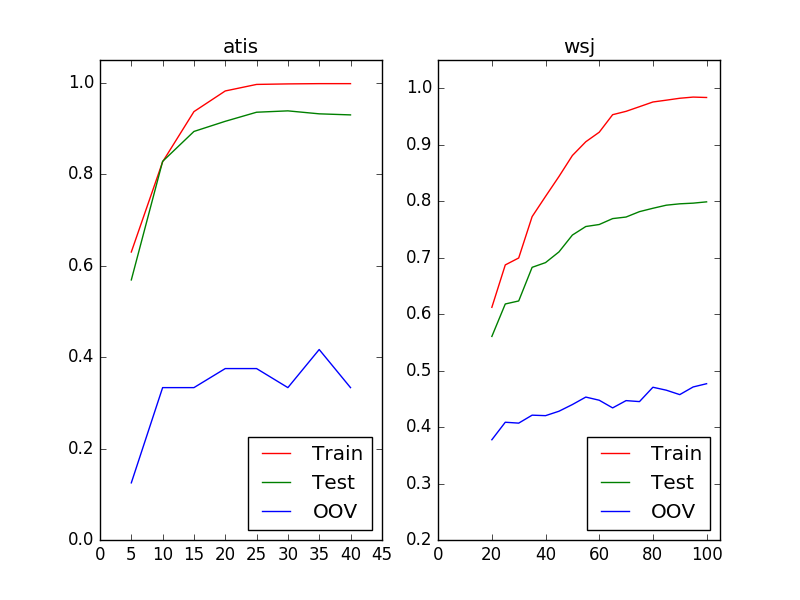
\includegraphics[width=0.95\columnwidth]{figs/iterations}
\caption{Plot of of CRF's accuracy as a function of the number of iterations.}
\label{fig:iterations}
\end{figure}

\subsection{Effect of number of iterations}
HMM's inference procedure, being based on frequency counts, is not iterative. However, CRF uses an iterative optimization procedure to learn optimal weights. Fig. \ref{fig:iterations} shows the plot of accuracy of CRF on atis and wsj as the number of iterations are varied. As expected, all three accuracy metrics show a general increasing trend as the number of iterations are increased, though accuracy on OOV words seems to wander a bit.

\subsection{Adding features directly to POS-tags}
HMM does not directly support additional features. One way to emulate feature addition is to modify the POS-tag set by including features in the tag itself. For example, ``Flying'' is tagged with \texttt{VB-caps-ing}, instead of \texttt{VB} with features \texttt{-caps, -ing}. Table. \ref{table:modified} summarizes the result of running HMM and CRF on this modified POS-tagged dataset. The accuracy of both HMM and CRF drop because the modified POS-tag set becomes huge ($282$ POS-tags on wsj, up from $45$) and brings about data sparsity. Moreover, in CRF, not only does the modified tag-set \emph{not} emulate additional features, it makes inference harder. CRF on wsj with modified tag-set had not converged in about 13.5 hours, having completed only 19 iterations.

\end{document}
